
\subsection{PARTICLE IMAGE VELOCIMETRY}

$PIV$ is a technique to determine the  velocity field of objects from a stream of images\cite{Bastiaans}.
The result of the $PIV$ is given as a vector field, showing for each particle the direction, sense and intensity of velocity. 
Moreover, the $PIV$ can be used for different objects in the same image.
For this purpose, the $PIV$ technique divides the frame 1 in possibles regions where target can be found, 
after frame 1 and 2 are correlated using comparative method, so a vector or a field of vector is generated 
starting of initial point till final point. Thus, we have displacement and time of computing, applying of 
conception of derivate it is possible to estimate relative velocity.

\begin{figure}[H]
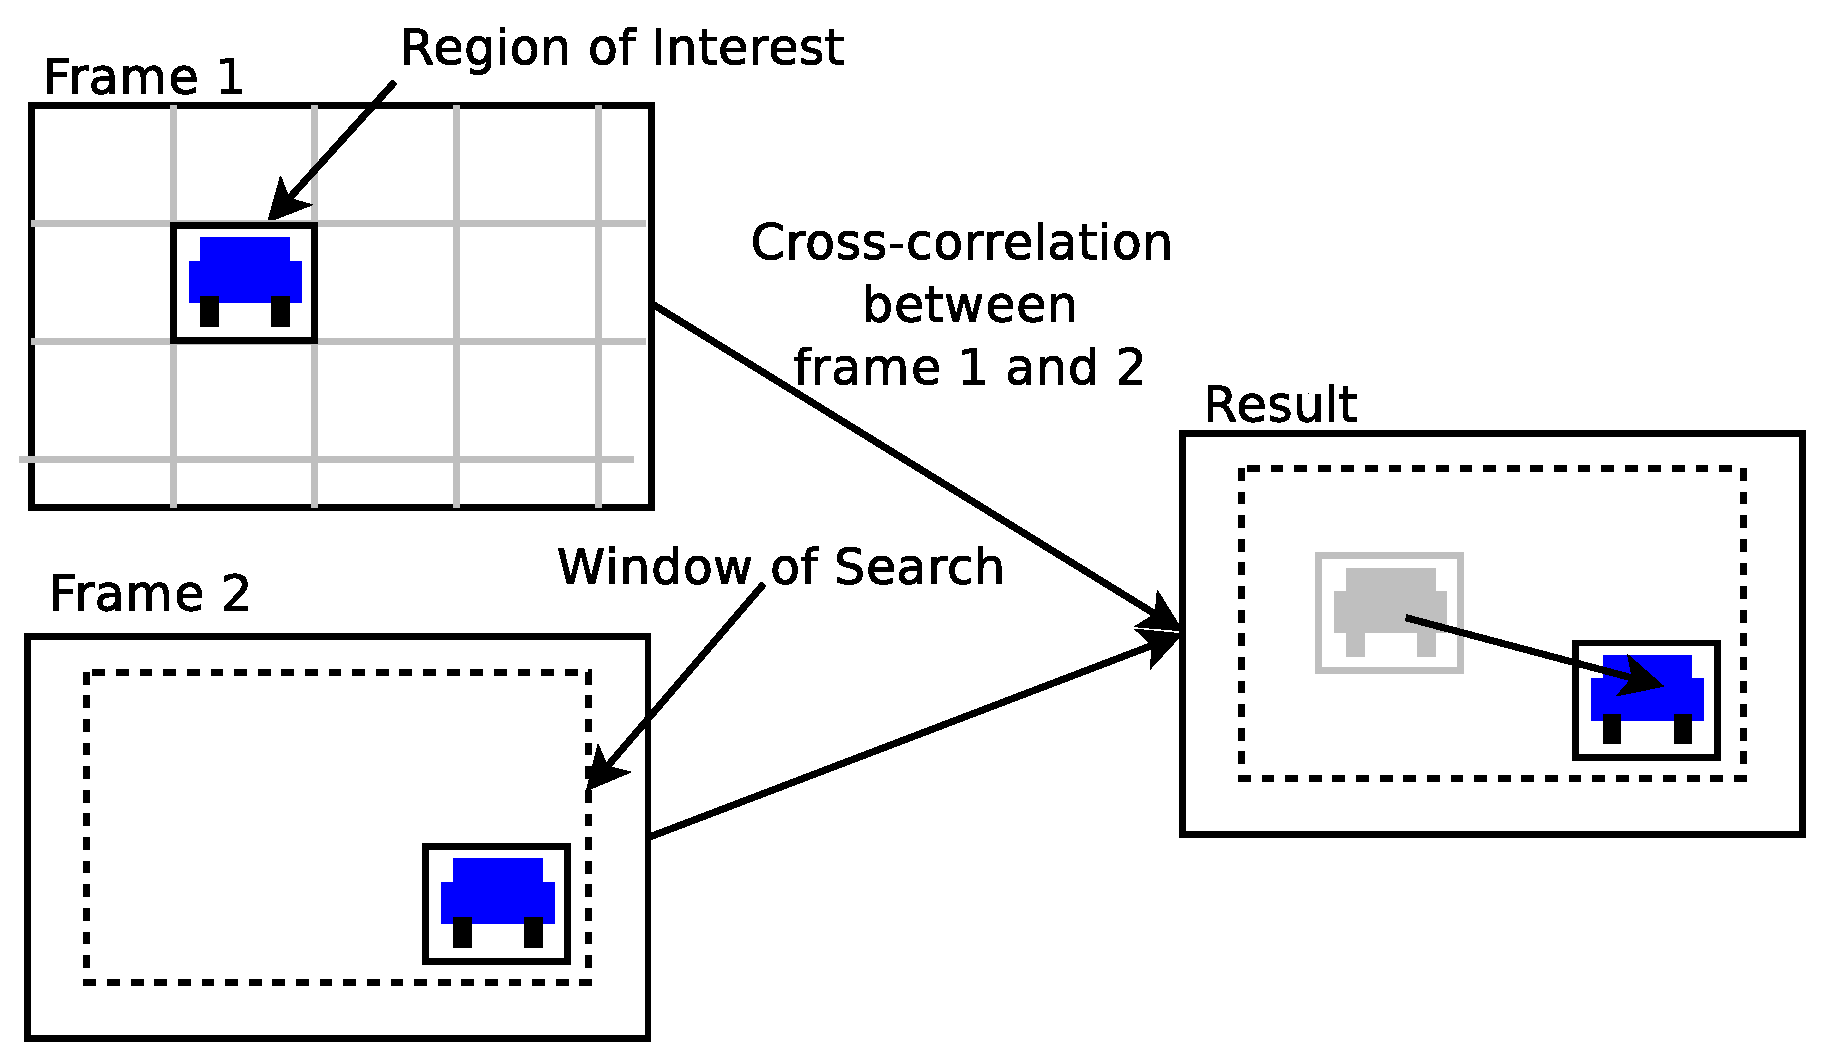
\includegraphics[width=\columnwidth]{images/explanationPIV.eps}
\caption{The PIV operation comparing two frames}
\label{fig:twoframes}
\end{figure}

The Fig. \ref{fig:twoframes} illustrates how PIV works and demonstrates the relation between Region of Interest (ROI) and 
Window of Search (WOS). WOS is region where target can be found and consequently WOS must involve ROI. 
WOS doesn't fill necessary whole image. If WOS is large, we have an augment of computing but 
if WOS is too small, target in high velocity has more chances to be lost. In our application, 
we determine WOS from 1,5 of ROI. For example, if ROI is 200x300 so we have WOS of 300x450. 
It means target will be in anywhere in this WOS. This consideration can be
proven by testes in environment of low velocity of objects (permitted velocity in cities and roads).

\begin{figure}[H]
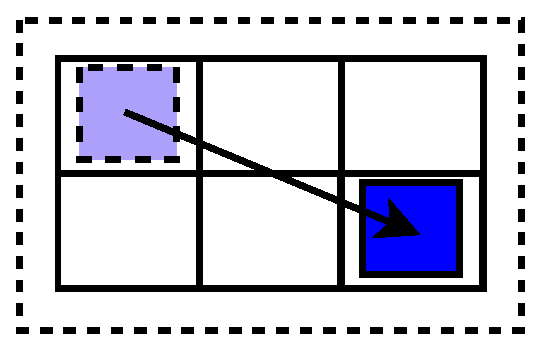
\includegraphics[width=\columnwidth]{images/WOSdivided.eps}
\caption{WOS is divided in windows of same dimensions of ROI}
\label{fig:WOSdivided}
\end{figure}

ROI is one of most important part of PIV, because it contains target. An window of same dimension of ROI is displaced
along of whole WOS in frame 2, like showed in Fig. \ref{fig:WOSdivided}. Comparisons are done among frames and 
assigned a value. 
When process finishes, the more height value refers the new place of ROI. It means that target displaced of a point in 
frame 1 to another in frame 2.